\chapter{Evaluation}

\begin{figure}[hbtp]
	\centering
	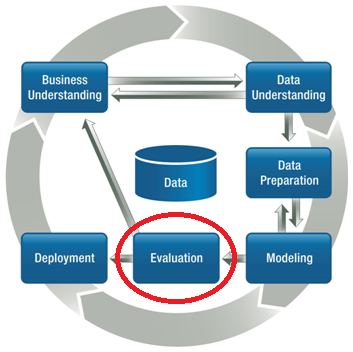
\includegraphics[width=0.5\textwidth]{./images/CRISPDM_5.png}
	\caption{CRISP-DM - Evaluation}
	\label{CRISPDM_5}
\end{figure}

In questa fase si andranno a valutare i risultati ottenuti dall'intero processo CRISP-DM fatto finora. Se tale valutazione risulta essere non positiva rispetto a ciò che il sistema si prefiggeva di fare, si passerà alla definizione di altri parametri o alla scelta di altri tipi di algoritmi per effettuare il campionamento.

\section{Valutazione rispetto agli obiettivi di business}

I risultati ottenuti rispettano gli obiettivi di business definiti al capitolo \ref{task}, in quanto supera il 99 \% di correttezza. però sono state fatte altre prove cambiando il ft in ft leaves e ft inner. in seguito i risultati.
\section{Raccomandazioni per revisioni future}
